% pre-amble section
\documentclass[11pt,english]{article}
\usepackage[utf8]{inputenc}
\usepackage{babel}
\usepackage{hyperref}
\usepackage{graphicx}

\title{Herbert\\Autonomous Robotic Rubik's Cube Solver}
\author{
    Jonathan Whitaker\\
    \textt{jon.whitaker@utah.edu}
    \and
    Dylan Lytle\\
    \textt{dylan.lytle@utah.edu}
    \and
    Matt Frandsen\\
    \textt{matt.frandsen@utah.edu}
    \and
    Li Lao\\
    \textt{li.lao@utah.edu}
}
\date{April 2015}
% end of pre-amble

% document content
\begin{document}

\maketitle

\tableofcontents

\section{Abstract}
Project Herbert is an autonomous robotic Rubik's Cube solver that is composed of a complex network of mechanical and electrical devices. In this project our team will be interfacing with these complex mechanical and electrical devices so as to design and create an autonomous robot that is capable of achieving record-breaking Rubik's Cube solution sequences.  This project will be an integration of various technologies including: mechanical actuators, electrical stepper motors, single-board computers, field-programmable gate arrays (FPGAs), and video cameras. 

\section{Introduction}
The purpose of this project is to create an autonomous robotic Rubik's Cube solver through the integration of several components. The main components needed in our project include video cameras, electrical stepper motors, mechanical actuators, a single-board computer, and an FPGA. The video cameras connect to the computer through standard USB 2.0 protocol \cite{USB 2.0}. The video cameras are responsible for capturing the initial configuration of the Rubik's Cube, and the single board computer is responsible for processing the video frame information and generating a matrix model for the initial state of the cube. After generating a matrix model for the initial cube, the computer will then apply Kociemba's algorithm \cite{Kociemba} (an optimal algorithm used to solve a Rubik's Cube) to generate a solution sequence that can be processed sequentially. The solution sequence that Kociemba's algorithm will return will be in the standard notation used in Rubik's Cube discussion and theory (see \ref{sec:Kociemba}). As each solution sequence is processed, the computer will communicate through an RS232 serial connection to an FPGA board which will drive the mechanical actuation and stepper motor rotations needed to physically manipulate the cube. The FPGA will act as a system control board and will be responsible for controlling the actions of two motor control boards and a relay board used to trigger the mechanical actuators. An overview of this process can be found below in 'fig here' of section \ref{sec:Project Design}.

\section{Project Design}
\label{sec:Project Design}

\begin{figure}[!ht]
\centering
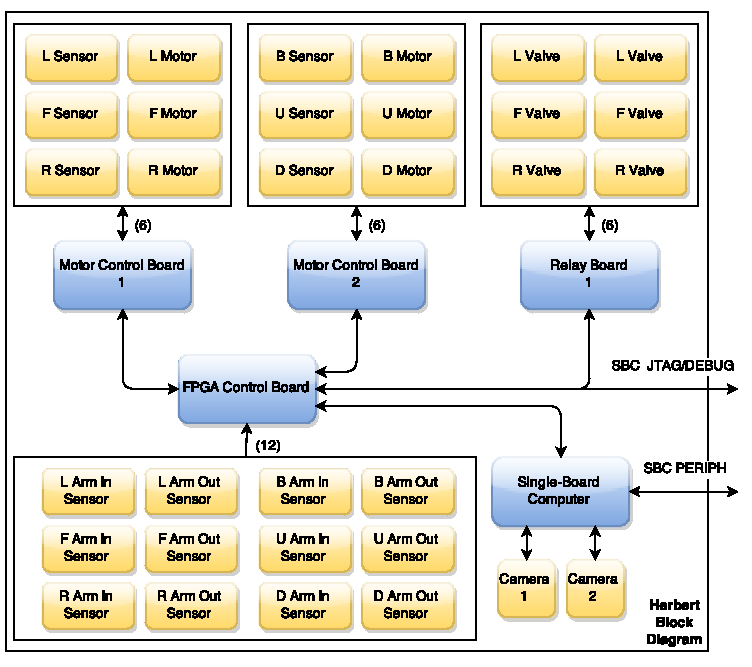
\includegraphics{Herbert System Diagram.pdf}
\caption{Herbert Block Diagram}
\label{fig:System Block Diagram}
\end{figure}

\subsection{Capturing the Cube with OpenCV}
\subsection{Kociemba's Algorithm and the Solution Sequence}
\label{sec:Kociemba}

\section{Schedule}
\section{Required Resources}
\section{Summary}
\section{Bibliography}
\begin{thebibliography}{9}
\bibliographystyle{IEEEtran}

\bibitem{USB 2.0}
\emph{USB 2.0 Specification}
[Online]. Available: \url{http://www.usb.org/developers/docs/usb20_docs/}

\bibitem{Kociemba}
Herbert Kociemba.
\emph{The Two-Phase Algorithm}
[Online]. Available: \url{http://kociemba.org/cube.htm}

\end{thebibliography}
\end{document}
% end of document content
